\subsection{Server}\label{archServer}
Per rendere lo sviluppo più semplice, e garantire la manutenibilità del codice il team ha optato per un approccio modulare. In questo modo, avendo moduli separati con compiti distinti, sarà più semplice modificarne o estenderne il comportamento senza dover necessariamente modificare la base comune.\\

\subsubsection{UML}
\begin{figure}[H]
	\begin{center}
		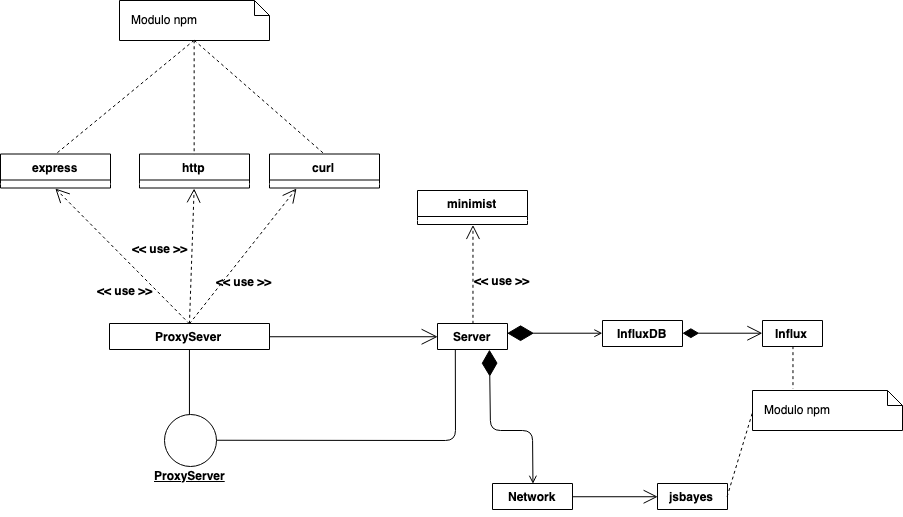
\includegraphics[scale=0.5]{./images/server_class_non_espanso.png} 
	\end{center}
	\caption{Architettura dell'applicativo}
\end{figure}

\begin{itemize}
 \item \textbf{Server}: è il modulo principale che si occupa della comunicazione dei vari moduli che compongono il server, e della gestione delle richieste provenienti 
 dai vari panelli;
 \item \textbf{InfluxDB}: è il modulo che si occupa di adattare la libreria \textit{Influx} e ci fornisce un set di metodi specializzati;
 \item \textbf{Network}: è il modulo che si occupa di adattare la libreria \textit{jsbayes} e costruisce la rete bayesiana da utlizzare;
\end{itemize}

\subsubsection{Descrizione delle Classi e dei Metodi del Pannello}\label{descrizionearchServer}

\paragraph{Server}

\begin{itemize}

	\item \textbf{constructor()}: costruttore di classe. Inizializza l'istanza di express\glossario , l'array di
	 connessioni, reti e di pool, inoltre esegue una verifica sintattica sui parametri di configurazioni passati 
	 tramite \textit{conf.json};

	 \item \textbf{configExpressApp()}: metodo utilizzato per l'inizializzazione delle varie route\glossario messe 
	 a disposizione dal server;

	 \item \textbf{parserNetworkNameURL(name)}: metodo utilizzato per parsare il nome di una rete 	
	 proveniente da indirizzo URL. 
	 Ritorna false in caso di errore o stringe non valide, altrimenti ritorna il nome parsato;

	 \item \textbf{saveNetworkToFile(data)}: metodo utilizzato per il salvataggio su filesystem delle reti 
	 bayesiane caricate dall'utente. Riceve come input un json rappresentate la rete bayesiana. Ritorna un 	
	 booleano a true se il salvataggio è stato eseguito o false altrimenti. Lancia eccezioni in caso di errori di 
	 scrittura su filesystem;

	 \item \textbf{startServer()}: metodo utilizzato per l'effettivo avvio del server. Mette in ascolto il server 
	 sulla porta configurata a costruttore ed inizializza le reti salvate su filesystem; 

	 \item \textbf{shutDown()}: metodo utilizzato per la chiusura del server; 

	 \item \textbf{initSavedNetworks()}: metodo utilizzato per  la lettura da file system e il successivo
	 caricamento in memoria  delle reti bayesiane salvate in filesystem. Per ogni rete letta, viene chiamato
	 il metodo \textit{initBayesianNetwork(net)};

	 \item \textbf{initDatabaseConnection(connection)}: metodo utilizzato per l'inizializzazione di una 
	 connessione al database. Riceve come parametro un json di definizione della connessione da creare. 
	 Può lanciare un'eccezione in caso di fallimento;

	 \item \textbf{initBayesianNetwork(net)}: metodo utilizzato per aggiungere un'istanza di \textbf{Network}
	 all'array di reti monitorate. Riceve in input la definizione della rete in json, e ne crea l'oggetto che la rappresenta; Può lanciare eccezioni. Ritorna true se la creazione è andata a buon fine; 

	\item \textbf{countNetworks()}: ritorna in numero di reti nell'array di reti monitorate; 

	\item \textbf{observeNetworks(net, data)}: metodo utilizzato per risolvere le dependency richiesta
	dall'oggetto \textit{Network} per eseguire il calcolo delle probabilità. Riceve in input la rete da osservare
	e i dati richiesti da quest'ultima. Successivamente esegue una chiamata al database chiedendo i dati 
	necessari al calcolo per poi eseguire i calcoli con quest'ultimi chiamando il metodo apposito. Inoltre 
	il metodo è incaricato della gestione delle soglie critiche modificando qualora fosse necessario 
	la politica temporale di ricalcolo. Fine richiama il metodo \textit{writeMesure(net)}; 

	\item \textbf{configParser()}: metodo utilizzato per il controllo  della sintassi nel file di configurazione.
	Ritorna true se la sintassi è corretta, false altrimenti; 

	\item \textbf{checkParam(argv)}: metodo utilizzato per il controllo dei parametri passati da terminale
	all'avvio del server. Ritorna true se i parametri sono validi, false altrimenti; 

	\item \textbf{getNetworks()}: metodo utilizzato per la creazione di un'array contenente il nome e 
	il campo \textit{monitoring} di tutte le reti salvate in filesystem. Ritorna un'array di tuple stringa, boolean; 

	\item \textbf{getMilliseconds(temporal)}: metodo utilizzato per la conversione della politica temporale in 
	ore, minuti, secondi in millisecondi. Riceve in input un json con ore, minuti e secondi definiti come interi, 
	e ritorna un intero, il quale rappresenta la conversione in millisecondi; 

	\item \textbf{addToPool(net)}: metodo utilizzato per aggiungere al monitoraggio una rete bayesiana già 
	caricata in memoria. Riceve come parametro il nome della rete, con quest'ultimo viene verificato 
	se è gia presente nel all'array di pool. Se non è presente viene aggiunto al pool seguendo le politiche 
	temporali riportate dall'utente. Ritorna true nel caso in cui la rete sia stata aggiunta con successo, false 
	altrimenti; 

	\item \textbf{deleteFromPool(net)}: metodo utilizzato per l'eliminazione di una rete in monitoraggio. Riceve
	come parametro il nome della rete. Se la rete è in monitoraggio viene fermata ed eliminata dal pool.
	Ritorna true se la rete è stata eliminata dal pool di monitoraggio, false altrimenti; 
	
	\item \textbf{writeMesure(net)}: metodo utilizzato per la scrittura delle probabilità calcolate dalla
	varie reti in monitoraggio sui rispetti database di salvataggio. Riceve in input il nome di una rete, 
	dopodiché preleva le probabilità calcolate dall'oggetto rappresentate la rete e le scrive sul database. 
	Ritorna true se i dati sono stati scritti con successo, false altrimenti; 
	
\end{itemize}

\paragraph{Network}
\begin{itemize}

	\item \textbf{constructor(net)}: costruttore di classe a un parametro. Riceve la definizione di una rete 
	bayesiana in formato JSON e ne costruisce l'oggetto rappresentate; 

	\item \textbf{observe(node, state)}: metodo utilizzato da wrapper\glossario per l'utilizzo del metodo 
	\textit{observe} della classe \textit{jsbayes}. Riceve in input due parametri: net	di tipo stringa e state di 
	tipo stringa; 

	\item \textbf{sample(n)}: wrapper del metodo \textit{sample(n)}, della classe \textbf{jsbayes}. 
	Esegue il calcolo delle probabilità dei vari nodi con il metodo \textit{Monte Carlo}. Riceve in input un 
	numero intero il quale indica il numero di iterazioni da eseguire; 
	
	\item \textbf{unobserveAll()}: metodo utilizzato per togliere dall'osservazione i vari nodi precedentemente 
	collegati. Per ogni nodo viene richiamato il metodo \textit{unobserve(node)} della classe jsbayes; 
	
	\item \textbf{orderTresholds()}: metodo utilizzato per il riordinamento delle soglie, in ordine crescente e 
	decrescente, definite nella rete; 
	
	\item \textbf{observeData(dati)}: metodo utilizzato per l'osservazione dei dati. Riceve in input un'array 
	associativo dei dati necessari da monitorare, tramite i quali verranno effettuate a seconda delle 
	soglie, i confronti tra dati - soglie, per poi successivamente fare scattare la probabilità con li metodo 
	\textit{observe}. In finte una volta eseguiti tutti i confronti verrà richiamato il metodo \textit{sample} per 
	calcolare le probabilità. Ritorna true se una soglia critica è stata superata, false altrimenti; 
	
	\item \textbf{getProbabilities()}: metodo utilizzato per estrarre le probabilità di ogni stato, per ogni 
	singolo nodo. Ritorna un'array associativo con il nome del nodo e un array contenete le probabilità. 
	Quest'ultimo a sua volta è un'array associativo formato da tuple: nome stato e probabilità calcolata; 
			
\end{itemize}

\paragraph{InfluxDB}

\begin{itemize}

	\item \textbf{constructor(host, port, database, dbwrite, user, pwd)}: costruttore di classe. Riceve in 
	input host e porta sulla quale il database è in ascolto, il nome del database, il database sul quale salvare i 
	dati, username e password. Il metodo costruisce un oggetto \textit{Influx} il quale rappresenta la 
	connessione al database. Avviene un controllo dei dati passati input con opportuno lancio di eccezioni 
	nel caso in cui alcuni dei dati non fossero conformi alla sintassi o errati; 
	
	\item \textbf{getDatasources()}: metodo utilizzato per estrapolare le tabelle disponibili per la lettura.
	Ritorna una \textit{Promise}\glossario da risolvere successivamente. Può lanciare un'eccezione nel caso in cui 
	la query\glossario al database fallisca o sia interrotta; 
	
	\item \textbf{queryDB(query)}: wrapper del metodo \textit{query} della classe \textit{InfluxDB}, il quale
	viene utilizzato per l'interrogazione del database tramite query; 
	
	\item \textbf{getDatasourcesFields(source)}: metodo utilizzato per estrarre le colonne di una determinata 
	tabella. Riceve in input una source da ispezionare. Ritorna una \textit{Promise} da risolvere
	successivamente; 
	
	\item \textbf{getLastValue(source, field)}: metodo utilizzato per leggere l'ultimo dato in serie temporale 
	dal database. Riceve in input la source dalla quale estrarre il field interessato. Ritorna una 
	\textit{Promise}
	da risolvere successivamente. Può lanciare un'eccezione nel caso in cui l'interrogazione del database 
	fallisca; 
	
	\item \textbf{getListData(fields)}: metodo utilizzato per generare un'array di ultimi dati, prelevati 
	in serie temporali dal database. Riceve in input un'array di json, nel quale per ognuno di essi viene 
	definito un campo table ed un campo flush. Per ogni valore da prelevare viene richiamato il metodo 
	\textit{getLastValue} per ricevere l'ultimo dato in ordine temporale. 
	Ritorna un'array di tuple: nome campo  e valore campo; 
	
	\item \textbf{writeOnDB(net, probs)}: metodo utilizzato per la scrittura delle probabilità di una rete sul
	database di scrittura definito in fase di costruzione. Riceve in input il nome della rete e le sue probabilità. 
	Per ogni nodo della rete viene inserito un campo contenente il nome del nodo e le varie probabilità
	calcolate; 
	
	\item \textbf{checkStatus(timeout)}: metodo utilizzato per verificare la connessione al database. 
	Riceve in input un timeout utilizzato per effettuare un ping\glossario al database ogni 
	\textit{timeout} secondi. Ritorna un \textit{Promise} da risolvere successivamente la quale 
	contiene i dati di risposta dal database; 

\end{itemize}








